%File: formatting-instruction.tex
\documentclass[letterpaper]{article}
\usepackage{aaai}
\usepackage{times}
\usepackage{helvet}
\usepackage{courier}
\usepackage{graphicx}
\usepackage{wrapfig}
\usepackage{listings}
\usepackage{color}
\usepackage{float}

\frenchspacing
\setlength{\pdfpagewidth}{8.5in}
\setlength{\pdfpageheight}{11in}
\pdfinfo{
/Title (ELSEWeb meets SADI: Supporting Data-to-Model Integration for Biodiversity Forecasting)
/Author (Nicholas Del Rio, Natalia Villanueva-Rosales, Deana Pennington, Karl Benedict, C.J. Grady, Aimee Stewart)}
\setcounter{secnumdepth}{2}  

\begin{document}
% The file aaai.sty is the style file for AAAI Press 
% proceedings, working notes, and technical reports
%
\title{ELSEWeb meets SADI: Supporting Data-to-Model Integration for Biodiversity Forecasting}
\author{Nicholas Del Rio\textsuperscript{1}, Natalia Villanueva-Rosales\textsuperscript{1}, Deana Pennington\textsuperscript{1}, Karl Benedict\textsuperscript{2}\AND Aimee Stewart\textsuperscript{3}, C.J. Grady\textsuperscript{3}\\ 
Cyber-Share Center of Excellence, 500 W University Ave, El Paso, TX 79968\textsuperscript{1}\\
Earth Data Analysis Center, MSC01 1110, 1 University of New Mexico, Albuquerque, NM 87131\textsuperscript{2}\\
University of Kansas Biodiversity Institute, 1345 Jayhawk Blvd., Lawrence, KS, 66045-7593\textsuperscript{3}
}
\maketitle
\begin{abstract}
\begin{quote}
In this paper, we describe the approach of the Earth, Life and Semantic Web (ELSEWeb) project that facilitates the discovery and transformation of Earth observation data sources for the creation of species distribution models (data-to-model) transformations. ELSEWeb automates the discovery and processing of voluminous, heterogeneous satellite imagery and other geospatial data available at the Earth Data Analysis Center to be included in Lifemapper Species Distribution models by using AI knowledge representation and reasoning techniques developed by the Semantic Web community. The realization of the ELSEWeb semantic infrastructure provides the possibility of combinatoric explosions of scientific results, automatically generated by orchestrations of data mash-ups and service composition. We report on the key elements that contributed to the ELSEWeb project and the role of automated reasoning in streamlining the Species Distribution Model generation and execution.
\end{quote}
\end{abstract}

\section{Introduction}
Scientists who study biodiversity are grappling with understanding potential climate and human impacts on biodiversity \cite{barnosky2011has}. There is much uncertainty involved - in what changes are likely to occur, how those changes interact with species, and how species interact with each other. In recent years numerous scientific efforts around the world have generated data and models necessary for biodiversity analyses. Indeed, there is a plethora of data and models to choose from, each with unique characteristics. There have been concerted efforts to standardize data and models to achieve interoperability. In particular, the Global Biodiversity Information Facility (GBIF; http://www.gbif.org) was established by governments in 2001 to provide access to species observation data. Similarly, the Group on Earth Observations (GEO; http://www.earthobservations.org) is a partnership of governments and international organizations creating a System of Systems (GEOSS) that aims to connect Earth observation data and tools. The GEOSS Model Web is an envisioned infrastructure to facilitate easy integration of data and models \cite{geller2008looking,nativi2012environmental}. Yet progress is slow, much of the legacy data remain difficult to discover, and the relevant environmental data are often voluminous, heterogeneous, and require specialized expertise to work with. Scientists who desire to conduct a particular analysis still typically use the tools they are already familiar with and invest much of their research time collecting or finding relevant data, preprocessing those data into forms that can be input into their tools, and manually integrating data and models. Hence, the significant amount of work involved means that they commonly conduct their analyses using a specific set of assumptions, data, and parameterizations based on the requirements of a single model. A better characterization of uncertainty could be achieved by iterating over many combinations of data, models, and parameterizations. The goal of the Earth, Life, and Semantic Web (ELSEWeb) project was to enable scientists to easily conduct these kinds of iterative analyses - creating an infrastructure for them to employ ``If-Then-ELSE'' mechanisms in their research (e.g., on-the-fly hypotheis testing and result comparison).

\section{Earth, Life, and Semantic Web}
The Earth, Life and Semantic Web (ELSEWeb) project was funded in 2012 through the NASA ACCESS program. ELSEWeb integrates Web services for data discovery, analysis, and delivery at the University of New Mexico Earth Data Analysis Center (EDAC; http://edac.unm.edu) with Web services at the University of Kansas for species distribution modeling (Lifemapper; http://lifemapper.org; LmSDM). EDAC is a data provider that specializes in satellite imagery and GIS data, and provides numerous web-service based data transformation tools. LmSDM is a set of web services that project potential future species distributions, see Figure \ref{fig:lifemapper-model}, from specimen occurrences and environmental data such as bioclimatic data derived from Worldclim (http://www.worldclim.org) and the International Panel on Climate Change (IPCC) climate models (e.g. temperature, precipitation). LmSDM lacked the ability to easily incorporate user-selected environmental datasets (land cover, soil type, water depth) into the analysis. These datasets are typically remotely-sensed satellite imagery or other environmental data. Users must locate relevant environmental datasets, prepare them in whatever way necessary for ingestion into Lifemapper, and manually upload them into LmSDM. A key feature of EDAC and Lifemapper is the use of open standards at both sites, creating the opportunity for automated data to model integration if the disparities between EDAC data and Lifemapper requirements could be identified and dealt with systematically.

\begin{figure}
\center
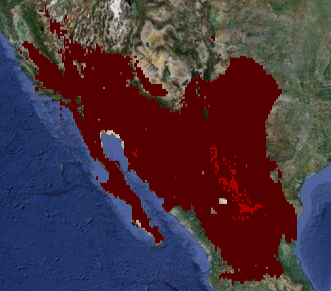
\includegraphics[width=50mm]{images/lifemapper-model.png}
\caption{Projected distribution of Larrea tridentata (dark red) modeled from environmental characteristics at known occurrence points (orange) using Services available at Lifemapper}
\label{fig:lifemapper-model}
\end{figure}

\subsection{Use Case}
The use case currently supported by ELSEWeb is discovery and transformation of data at EDAC that 1) covers a region of interest by place name or geographic coordinates; 2) is derived from particular instruments; and 3) has a particular semantic data type. These semantic data types, programmatically inserted as thematically defined keywords into the metadata published by EDAC, are a key element for enabling ELSEWeb and are not currently specified as components in the community service or data metadata standards, for example Open Geospatial Consortium (OGC, http://www.opengeospatial.org/) or Federal Geographic Data Committee (FGDC, http://www.fgdc.gov/metadata). Nevertheless, any data provider that reuses the semantic data types at EDAC or maps their own semantic data types to EDAC's could easily be integrated into the ELSEWeb system. More information about the semantic metadata extensions are described in the next section. At Lifemapper, ELSEWeb enables streamlined ingestion of a range of data types to supplement the bioclimatic change data already available. The bioclimatic data that Lifemapper uses have been preprocessed from raw climate change data to generate more biologically meaningful data. For instance, many species are constrained by the minimum nighttime temperatures. If a region is too cold at night during winter, species cannot survive. But the semantic meaning of ``winter'' is not based on a time of year; rather, it varies depending on global location. Hence, data discovery and integration based on the desired characteristics (e.g. coldest/warmest month, or wettest/driest month) rather than time of year requires the use of semantic descriptions. 

\subsection{Earth Data Analysis Center Data}
EDAC's large collection (over 280,000 individual datasets comprising over 1 billion features) of environmental and geospatial data are made available as OGC Web Map, Web Feature and Web Coverage Services (WMS, WFS and WCS respectively), which are REST-like web services accessible using HTTP Get requests. The published WCS services are the focus of the data publication capabilities supported in the ELSEWeb project. In general, WCS services advertise capabilities in a GetCapabilities XML document that describes the data layers (coverages) available for download, the region encompassing the data layers and the different formats in which the data can be returned (e.g., PNG, JPEG, and TIFF). From the GetCapabilities XML, clients are able to create URLs that specify what data layer is being requested, the subregion that should be returned, any resampling or coordinate transformation that should be performed, and how the returned data should be encoded. Although GetCapabilities XML describes many of aspects of the data needed to support our use case, the information is not specified at a semantic level and therefore may not be easily integrated with other non-OGC specific datasets using different nomenclature; this syntactic limitation is elaborated on in the following section. Upon submission of a WCS request URL, services return the specified data in a multipart MIME format, as per the specifications set forth by OGC. These multipart mime messages contain two parts: an XML metadata description of the data returned (e.g., size and encoding) and the actual data payload.
 
The GetCapabilities XML schema was designed to be extendable in order to allow publishers to describe additional metadata pertinent for specific domains. For example, service publishers can include information such as the semantic type of the data layers, the duration the data was collected as well as the sensor responsible for collecting the data if the data are remotely sensed. In particular, EDAC currently publishes metadata using the Federal Geographic Data Committee (FGDC) \cite{federal1998fgdc} metadata standard to describe both the semantic type of the data as well as information about the collecting instrument (e.g., sensor) and provides links to these metadata from the GetCapabilities XML document. The FGDC metadata extensions are associated with the OGC Web Services XML element: ogc:Metadata. Semantic data type descriptions are expressed using the Climate Forecast (CF, http://cf-pcmdi.llnl.gov/) terminology and these semantic descriptions are referenced from within the FGDC metadata title element \cite{eaton2003netcdf}. Therefore, EDAC employs a family of three metadata standards to describe their WCS services: OGC GetCapabilities XML, FGDC, and CF. Looking forward, EDAC has implemented support for the ISO 19115, 19110, and 19119 set of data and service metadata standards as a complement to the standards currently supported for the ELSEWeb project. 


\subsection{Lifemapper Experiment Requirements}
Lifemapper modeling is also available as a RESTful service accessible using HTTP Post. The  interface to Lifemapper is well defined using the Web Application Description Language (WADL), which describes the input and output schema of the XML HTTP payloads.  The basic constructs of the Experiment.xml is composed of a ``Scenario Layer Set'', consisting of references to TIFF environmental data such as temperature or rainfall; passing by reference is a useful technique in order to keep message payloads from exploding because of base64 encoding of binary data. An experiment also specifies species occurrence data whose predicted distribution will be calculated from the environmental scenario specified. Finally, the specific modeling algorithm that will be used to calculate the predicted distribution, such as BIOCLIM \cite{busby1991bioclim}, is specified.

After successful submission of an experiment, Lifemapper generates a species distribution model (SDM) and predicted species distribution map and returns a URL referencing the newly generated SDM metadata and map. The model is processed with one set (observed climate), the projections (observed and future predicted climate) with 10 sets for totals of approximately 300GB and 3TB, which can be considered ``Big Data''. Outputs are 1.5GB each. The map can be returned from the Lifemapper website as an image, shown in Figure \ref{fig:lifemapper-model} using OGC Web Mapping Services (WMS), or imported into Quantum GIS (QGIS; http://www.qgis.org) and VisTrails (http://www.vistrails.org) systems using the Lifemapper plug-in support. QGIS supports scenarios such as when users want more sophisticated visualizations than the default map images, to examine the data, or perform additional operations on the SDM such as aggregations with other models and statistical analyses.

\subsection{Challenges to Generate Lifemapper Models using EDAC Data}
The disparity between the (1) forms of available EDAC data and (2) Lifemapper data ingestion requirements requires a more sophisticated process than data discovery alone. Note that the data returned from EDAC's WCS services cannot be directly referenced as a scenario layer set due to the multipart message format that is not supported by Lifemapper. The ELSEWeb integration, described in the next section, extends discovery and introduces data aggregation, sequencing, and format transformations which are operations necessary for appropriately structuring EDAC WCS service responses to satisfy Lifemapper data requirements. 

\begin{figure*}
\center
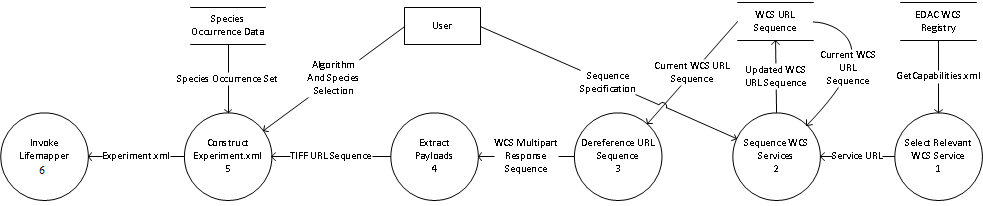
\includegraphics[width=170mm]{images/elseweb-workflow.png}
\caption{The workflow that streamlines EDAC data into Lifemapper modeling services}
\label{fig:elseweb-workflow}
\end{figure*}

Figure \ref{fig:elseweb-workflow} highlights the necessary transformations required to structure EDAC gridded WCS data into scenario layer sequences required by Lifemapper:

\begin{small}
\begin{enumerate}
\item Search through (thousands of) WCS services provided by EDAC and identifying a relevant subset:
    \begin{enumerate}
	\item Reading through XML if metadata is exposed in its raw form
	\item Mapping states and geographical regions to latitude and longitude bounding boxes
	\item Reading through cryptic satellite/sensor labels
	\item Reading through date ranges, possibly confounded within the label of the service name itself
	\end{enumerate}
\item Generate a WCS calling sequence
\item Execute each selected WCS service
\item Extract data payloads from the multipart messages
\item Construct Lifemapper Experiment.xml
    \begin{enumerate}
    \item Select species occurrence set
    \item Select algorithm
    \item Embed reference to TIFF URL Sequence (i.e., scenario layers) 
	\end{enumerate}
\item Invoke Lifemapper by requesting an SDM provided the Experiment.xml
\end{enumerate}
\end{small} 
 
Although these tasks could be hard-coded into a workflow, the resulting software may not be easily extendible to include other data sources or other model providers. If the workflow was extended to include other data sources or models, the resulting specification may become complex and difficult to maintain due to the high number of various data formats and modeling capabilities currently published on the Web. One goal of ELSEWeb is to provide scalable solutions for other providers (e.g, data or models) that might wish to ``plug-in'' into ELSEWeb infrastructure. In order to develop an infrastructure that accommodates this flexibility, we turned to semantic web technologies that can be configured to automatically mitigate disparities between data providers and modeling services.

\section{The ELSEWeb Approach}
ELSEWeb enables LmSDM users to automatically integrate EDAC data into SDMs using the Semantic Automated Data Integration framework (SADI; http://sadiframework.org) \cite{wilkinson2011semantic} to support the specific task of automatically transforming data from EDAC to fit input requirements of Lifemapper. 
\begin{figure}[H]
\center
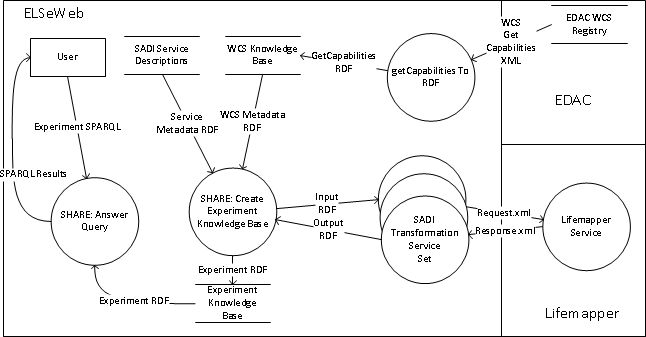
\includegraphics[width=90mm]{images/elseweb-flow.png}
\caption{Data flow representation of the ELSEWeb infrastructure}
\label{fig:elseweb-flow}
\end{figure}


Users in ELSEWeb request for the generation of species distribution models by specifying SPARQL \cite{prud2008sparql} queries, which are satisfyied by the SHARE client \cite{vandervalk2010share} provided by the SADI framework. SHARE executes ELSEWeb SADI services and aggregates resulting RDF output to compose an Experiment knowledge base, which contains the information needed to answer a specific SPARQL query. SHARE relies on the ELSEWeb knowledge base that contains SADI service descriptions that wrap EDAC and Lifemapper services in order to formulate service execution plans that will generate the minimal subset of RDF needed to satisfy a specific query. The use of the SADI framework is further detailed in the following subsections.

\subsection{Data Discovery and Mashup with the SADI Framework}
The ELSEWeb project leveraged the SADI framework to expose services providing data and modeling services from EDAC and SDM services from Lifemapper. SADI uses standards-compliant Web languages and Semantic Web service patterns to exchange RDF resources \cite{wilkinson2011semantic}. SADI services are defined in terms of the input and output class descriptions using the Web Ontology Language (OWL) \cite{mcguinness2004owl} corresponding to the instances they consume and produce respectively. Every service provides explicit relations between the output data and the input data through RDF properties. The SADI framework includes APIs and plug-in tools to facilitate the generation of these services by non-programmers, e.g., the SADI Taverna plug-in \cite{withers2010semantically} and the Protege plug-in \cite{wilkinson2010sadi}. SADI has been used in the biomedical domain, in particular, to enable data integration for personalized medicine \cite{vandervalk2010share,vandervalk2013sadi} and the integration of biological data \cite{riazanov2012ecotoxicology,callahan2013ontology}. 

To exemplify our use of SADI in ELSEWeb, consider the Extract Payloads activity that extracts TIFF payloads from EDAC WCS service responses. In our workflow diagram, the input to payload extraction is a sequence of WCS service request URLs and the output is a sequence of TIFF URLs. The SADI WCSPayload Extractor ingests {\tt WCSCoverage Sequences}, which are composed of (e.g., hasWCSCoverage) a sequence of maximum ten ordered {\tt WCSCoverages}. The {\tt WCSCoverage} class is elaborated on in Figure ref{fig:wcscoverage-owl}. Provided input, WCSPayload Extractor iterates through the {\tt WCSCoverage Sequence} and dereferences each WCS URL specified. The service then extracts the returned payload from the WCS responses and constructs the output {\tt WCSPayload Sequence}, which references ten URLs of the TIFF payload data that was extracted from the WCS responses.

\begin{figure}
\center
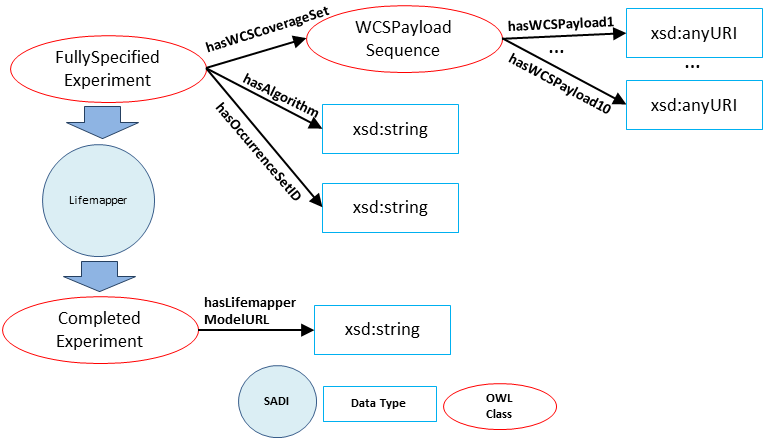
\includegraphics[width=90mm]{images/sadi-lifemapper.png}
\caption{Input and Output Interface of the SADI Lifemapper Service}
\label{fig:sadi-lifemapper}
\end{figure}

The Lifemapper SADI service, presented in Figure \ref{fig:sadi-lifemapper}, wraps the Lifemapper RESTful application. Lifemapper SADI service input is constrainted by the definition of the OWL class {\tt FullySpecifiedExperiment}, which specifies an algorithm name, and an ID of a species occurrence set. The Lifemapper SADI service extracts the required information from the input RDF and constructs the XML experiment request input for the Lifemapper RESTfull service. The SADI service also receives the response, which is a URL to a generated species distribution models, and creates the output RDF which in this case is an Experiment Stage 4, that simply references the SDM URL. Therefore, the SADI Lifemapper service encompasses both step 5 and 6 of the ELSEWeb workflow in Figure \ref{fig:elseweb-workflow}.

Other SADI services composing ELSEWeb are those that wrap the EDAC WCS services. These SADI services generate output RDF of type WCSCoverage, shown in Figure \ref{fig:wcscoverage-owl}. WCSCoverages specify what source or sensor recorded the data, the measurement type (i.e., semantic type) of the data, the bounding box region containing the data and the date the data was collected or recorded. Additionally, ELSEWeb contains a Sequencing service that constrcutes the WCS Coverage Sequence required by the payload extraction service. The input and output descriptions of our ELSEWeb SADI services comprise our WCS and SADI service knowledge bases presented in Figure \ref{fig:elseweb-flow}

\begin{figure}
\center
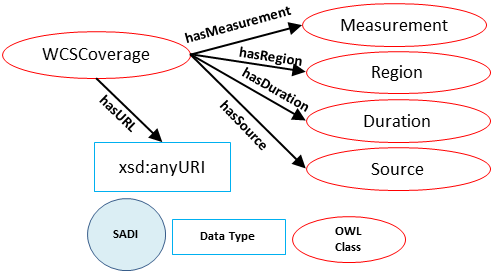
\includegraphics[width=70mm]{images/wcscoverage-owl.png}
\caption{A depiction of the WCSCoverage OWL specification of EDAC SADI service outputs}
\label{fig:wcscoverage-owl}
\end{figure}

\subsection{Service Orchestration using SHARE}
The SHARE client is a prototype tool provided by the SADI framework, which consumes SPARQL queries and maps each predicate (or relationship) involved in these queries to a SADI service that can provide such relation \cite{wilkinson2011semantic}. Each SPARQL query in ELSEWeb executes services for generating, aggregating and transforming data, creating models and explicitly asserting the relations between them in an ad-hoc manner via service orchestration. The SHARE client relies on a description logics reasoner for the automated service orchestration by accessing the ELSEWeb SADI registry. Although the SADI framework allows the registration of services into the global SADI registry, we opted for creating an ELSEWeb specific registry that currently contains only services supporting the required aggregations and transformations currently required by ELSEWeb and avoid the search through hundreds of SADI services from the biomedical domain registered in the global registry.

Below is an example ELSEWeb specific SPARQL query that requests for the generation of a Lifemapper model provided a set of experimental constraints. The experiment constraints define what WCSCoverages should be bound to each scenario layer, the algorithm that should be employed in Lifemapper, and the species occurrence ID. These constraints are defined in OWL and referenced in the query using the FROM clause (line 2). An interesting aspect of the SPARQL query is that users can remain devoid of any knowledge about the required transformations between EDAC and Lifemapper; they need only be concerned with {\em what} they want not, which in this case is a $?modelURL$. {\tt CompletedExperiment} (line 8) denotes an experiment that has been processed by Lifemapper and therefore has a property {\tt hasModelURL} that points to the URL of the resulting SDM.

\begin{lstlisting}[numbers=left,numberstyle=\footnotesize,basicstyle=\footnotesize]
SELECT ?modelURL
FROM <http://../experiment-1-v3.owl>
where
{
?experiment hasModel ?model.
?model a Model.
?model hasModelURL ?modelURL.
?experiment a CompletedExperiment.
}
\end{lstlisting}

The experimental constraints referenced by the SPARQL query are specified in the OWL ontology indicated in the FROM clause (experiment-1-v3.owl)\footnote{http://cybershare.utep.edu/ontology/elseweb/experiment-1-v3.owl} and specify what kind of data should be bound to what specific layer (1 through 10). For example, a user can use the properties of the EDAC data ontology\footnote{http://cybershare.utep.edu/ontology/elseweb/edac-v3.owl}, shown in Figure \ref{fig:wcscoverage-owl}, to specify that data for some environmental layer should be sourced from the MODIS sensor, reside within the {\tt Western United States} and recorded within some {\tt Duration1}, elaborated on below. Below is an example of a rule that defines the relevant characteristics of some data to occupy the first element of a WCSCoverage Sequence. The rules is specified in OWL and encoded using the Manchester Syntax \cite{horridge2006manchester}. The paper will continue to use Manchester Syntax for any rule encodings.

\begin{lstlisting}[basicstyle=\footnotesize]
Class: WCSCoverage1
  EquivalentTo:
    (hasDuration some Duration1)
    and (hasRegion some WesternUnitedStates)
    and (hasSource value MODIS)
\end{lstlisting}

Note the classe definitions below, {\tt Duration1} and {\tt WesternUnitedStates}, which are defined in terms of property value restrictions that effectively specify the time and space requirements for the data layer. {\tt Duration1} is defined in terms of a {\tt hasStartDate} and {\tt hasEndDate}, while {\tt WesternUnitedStates} is defined in terms of a bounding box by using necessary and sufficient restrictions through an equivalent OWL class definition.

\begin{lstlisting}[basicstyle=\footnotesize]
Class: WesternUnitedStates
  EquivalentTo: 
  (hasLeftLongitude some xsd:double[>= -130.0])
    and (hasLowerLatitude some xsd:double[>= 20.0])     
    and (hasRightLongitude some xsd:double[<= -100.0])
    and (hasUpperLatitude some xsd:double[<= 50.0])
    SubClassOf: 
      UnitedStatesRegion
\end{lstlisting}


The SHARE client can then search through the ELSEWeb SADI registry and identify any EDAC services that match these constraints. Logically speaking, SHARE will infer that any data offered by EDAC services that matches the selection criteria to be of type {\tt WCSCoverageForLayer1} and therefore considered as an element of some {\tt WCSCoverage Sequence}. The process is identical for specifying the other nine layers.

\subsection{Service Orchestration}
Now that SHARE can identify the relevant data to bind to each layer and thus compose a {\tt WCSCoverageSequence}, it needs to figure out how structure the set of identified layers into a payload sequence. Focusing on the two SADI services presented earlier, it will be illustrated how the output of the payload extractor service can be used to create the {\\tt FullySpecifiedExperiment} that is required by the Lifemapper SADI service.
 
Consider the following rules (1) and (2) specified in our ontology that describes our service intputs and outputs:

\begin{lstlisting}[basicstyle=\footnotesize]
Rule1
Class: UnderspecifiedExperiment
  EquivalentTo: 
    hasWCSCoverageSet some WCSCoverageSequence
\end{lstlisting}

\begin{lstlisting}[basicstyle=\footnotesize]
Rule2
Class: FullySpecifiedExperiment
  EquivalentTo: 
    hasWCSCoverageSet some WCSPayloadSequence
    SubClassOf:
      UnderspecifiedExperiment
\end{lstlisting}

Rule 1 states that any individuals that have a {\tt WCSCoverageSequence} are considered to be of type {\tt UnderspecifiedExperiment}, meaning they are not ready for ingestion by Lifemapper. Rule 2 states that any individual that has a {\tt WCSCoveragePayload} are ready for Lifemapper processing and considered to be of type {\tt FullySpecifiedExperiment}. Assume that in the ELSEWeb knowledge base there exists an individual of type {\tt UnderspecifiedExperiment} (generated by other SADI service not discussed here for simplicity). Considering our example SPARQL query that requests for a {\tt CompletedExperiment}, SHARE must determine what sequence of services to execute in order to generate such an individual. SHARE knows about:

\begin{enumerate}
\item The SADI service input/output descriptions for PayloadExtractor and Lifemapper
\item The Service ontology that contains Rule 1 and Rule2
\item The target {\tt CompletedExperiment}, specified by the SPARQL query
\end{enumerate}
 
Based on these resources, SHARE can determine that it must eventually execute the Lifemapper service, since it outputs the requested {\tt CompletedExperiment} individuals. However, SHARE currently only knows about an {\tt UnderspecifiedExperiment} individual. Based on Rule 2, it can determine that the difference between an {\tt UnderspecifedExperiment} and a {\tt FullySpecifiedExperiment} is the range of the {\tt hasLayers} property. In order to infer an {\tt FullySpecifiedExperiment}, SHARE must invoke the WCSPayload Extractor service, since it transforms WCSCoverageSequences to WCSCoveragePayloads. Once the WCSPayload Extractor has executed, the returned WCSPayload Sequence RDF will trigger RULE 2 and reclassify the {\tt UnderspecifiedExperiment} as a {\tt FullySpecifiedExperiment} and thusly pass this experiment individual to the Lifemapper SADI service.


\subsection{Provenance in ELSEWeb}
Provenance is a trace of all of the data sources and analytical methods that were used in a scientific analysis or model. Provenance is of particular relevance here to trace the automated process carried out. ELSEWeb provenance enables users to visualize, query, and understand data sources at EDAC and Lifemapper; analytical methods used at EDAC to generate derived products; and parameters and analytical methods used within a Lifemapper computational experiment. ELSEWeb services extended the original SADI design to include provenance information about the service that generated the data and the parameters used (if any) using the PROV data model \cite{moreau2012prov}. ELSEWeb SADI services use the PROV Ontology (PROV-O) \cite{lebo2013prov}, which is a W3C recommendation to represent the PROV Data model using OWL. ELSEWeb provenance is presented in Figure \ref{fig:elseweb-prov}, in turn, promotes transparency and confidence in model outputs derived. Transparency is in particular importance in automated systems such as ELSEWeb where processes are not defined {\em a priori}.

\begin{figure}
\center
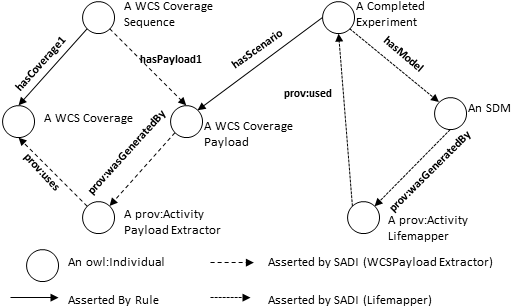
\includegraphics[width=80mm]{images/elseweb-prov.png}
\caption{Prov Trace from Lifemapper}
\label{fig:elseweb-prov}
\end{figure}


\section{Related Work}
The Model Web is founded on principles which dictate approachable methods for interaction with minimal barriers \cite{geller2008looking}. Therefore, ELSEWeb can be considered to implement a subset of the Model Web, in particular the Data-to-Model relationship, because users can quickly run experiments without any regard for how the data is sourced, aggregated, transformed and served to models. A similar contribution was made by the authors of eHabitat \cite{dubois2011ehabitat}, where a Habitat Irreplaceability Index (HRI) service was published as an OGC Web Processing Service (WPS) and integrated with WCS data, similar to EDAC. The eHabitat environment however lacks the semantic capabilities of ELSEWEb and so adding non-OGC compliant data sources or models may require manual reconfiguration of the workflows rather than delegating the transformational process to agents such as SHARE. The iPlant Semantic Web Platform uses SSWAP (Simple Semantic Web Architecture and Protocol) for the discovery of services and the construction and execution of workflows \cite{gessleriplant}. iPlant uses OWL ontologies and Resource Description Graphs (RDGs) to describe services, their inputs and their outputs. A difference between SADI and iPlant is that SADI describes services in terms of their input and output only, whithout creating a hierarchy of types of services. While SADI automatically orchestrates and executes service pipelines using a description logics reasoner, iPlant allows users to create pipelines through a graphical interface and uses a reasoner to suggest the next service in the pipeline according to the service descriptions. Similar to SADI, iPlant contains a knowledge base of services and their semantic annotations for the discovery and invocation of services that are executed by service providers over the web.   


\section{Discussion}
ELSEWeb leverages SADI best practices and lessons learned from other communities \cite{vandervalk2010share,vandervalk2013sadi,callahan2013ontology,riazanov2012ecotoxicology} and enables scientist to employ the ``If-Then-ELSE'' mechanism in their research. A key element in reusing and repurposing EDAC data and Lifemapper is the use of a family of metadata standards to describe their services. Service metadata is programatically created and can be automatically discovered and processed. ELSEWeb has been constructed in a generic way that allows for extensibility to other data and models as long as data and models are provided as services and defined following a standard-compliant format and language. 

SADI is agnostic to any particular ontology, as long as the RDF and OWL languages are used, reducing the knowledge negotiation process to an ontology mapping problem.


\section{Future Work}
{\bf Graphical Interface.} SPARQL can be seen as a workflow schema that will be used by the SADI framework to execute the services needed to obtain and transform data and models required by our user. We are in the process of creating a graphical interface that enables scientist to use the SHARE client without having to learn SPARQL or OWL to specify the experimental constraint considering two key variables for ELSEWeb: location and time. 

{\bf Expanding ELSEWeb services.} The vision of ELSEWeb includes the addition of services that provide additional data and models relevant to biodiversity forecasting. Ontology mapping will be used to align service descriptions and metadata. As a first step towards expanding ELSEWeb knowledgebase, services provided by the GEOSS registry \footnote{http://geossregistries.info/} will be analyzed for their addition through the SADI framework.  

{\bf Visualization.} ELSEWeb provides the possibility of combinatoric explosions of scientific results, automatically generated by orchestrations of data integrations and service composition yielding many different SDMs. An equally automated mechanism for helping users analyze the wealth of scientific products is needed and therefore we intend delegate the orchestration of visualization services to a reasoning engine tailored for pipeline composition \cite{del2012capturing}, similarly to how transformation orchestration is automated by SHARE.

Efforts similar to ELSEWeb to enable the automated publishing, discovery, and orchestration of services providing data and models will enable scientist to reuse data and test hypothesis on-the-fly using the "If-Then-ELSE" mechanism.

% insert KU Award number here as well
{\em\bf Acknowledgements} ELSEWeb is funded by NASA ACCESS grants NNX12AF49A (UTEP), NNX12AF52A (UNM). This work used resources from Cyber-ShARE Center of Excellence supported by NSF grant HRD-0734825 and HRD-1242122. The authors would like to thank Soren Scott and Bill Hudspeth from EDAC for their discussions about service metadata and the SADI development team for their steadfast support through their mailing list.



% ---- Bibliography ----
%
\begin{quote}
\begin{small}
\bibliographystyle{aaai}
\bibliography{elseweb}
\end{small}
\end{quote}
%
%


\end{document}
